\documentclass[journal]{IEEEtran}
\usepackage[utf8]{inputenc}
\usepackage[portuguese]{babel}


\ifCLASSINFOpdf
\else
   \usepackage[dvips]{graphicx}
\fi
\usepackage{url}

\hyphenation{op-tical net-works semi-conduc-tor}

\usepackage{graphicx}


\begin{document}

\title{Trabalho Genérico no formato IEEE}

\author{Don Ramón, Homer Simpson}

\markboth{Journal of \LaTeX\ Class Files, Vol. 14, No. 8, August 2015}
{Shell \MakeLowercase{\textit{et al.}}: Bare Demo of IEEEtran.cls for IEEE Journals}
\maketitle

\begin{abstract}
Este é o ambiente abstract. Aqui é feito um resumo do trabalho. Em geral o abstract não deve conter citações. Além disso, o texto deve ser redigido na terceira pessoa do singular, com o verbo na voz ativa, em linguagem clara, concisa e direta. A ABNT exige que o abstract seja de 150 a 500 palavras, porém sempre veja as instruções para o local onde você deseja enviar o seu trabalho. 
\end{abstract}

\begin{IEEEkeywords}
Normas, recomendações, trabalo acadêmico, UTFPR
\end{IEEEkeywords}


\section{Introdução}

Sempre leia as recomendações antes de redigir um trabalho para qualquer revista e/ou periódico \cite{pastro2019}. 

Para iniciar, veremos um logo da nossa universidade na Figura \ref{fig.UTFPR}.
\begin{figure}[h!]
	\centering
	\label{fig.UTFPR}
	
\includegraphics[width=.7\linewidth]{figs/UTFPR.png}
\end{figure}

\section{Referências da IEEE}
Uma boa dica para Engenharia Elétrica e afins é procurar referências em sites como \textit{IEEE Xplore}. Para exemplificar, entre nesse site:
\begin{verbatim}
	https://ieeexplore.ieee.org/document/8405897
\end{verbatim}

Caso você cite corretamente este trabalho, deve gerar uma referência como essa \cite{8405897}. Dica$^1$: verifique aqui e lá em baixo em \textit{References} para ver se você citou tudo certinho.

\section{Referência de outros lugares}

É comum encontrar citações úteis em trabalhos acadêmicos. Nesse caso, o ideal é procurar o trabalho que foi citado, para assim vermos a fonte original da informação. Por isso, cite esse trabalho \cite{torrico1999implementaccao}.

\section{Tabelas}

Tabelas são muito utilizadas para exibir informações de resultados. Por exemplo, veja a Tabela \ref{tab.generica1}:
\begin{table}[h!]
	\centering
	\begin{tabular}{|c|c|c|c|}
		\hline
		Cor        & Teste 1  & Teste 2                                           & Teste 3 \\ \hline
		Verde      & $\pi$    & \$\textbackslash{}frac\{\textbackslash{}pi\}\{2\} & $53$    \\ \hline
		Azul       & $\sigma$ & $2*\sigma$                                        & $55$    \\ \hline
	\end{tabular}
	\caption{Tabela genérica aleatória}
	\label{tab.generica1}
\end{table}

\section{Figuras Vetorizadas}

Uma dica muito importante é, sempre que possíve, utilizar figuras Vetorizadas. Exemplo de Figura vetorizada pode ser vista na Figura \ref{fig.vet}
\begin{figure}
	\centering
	\label{fig.vet}
	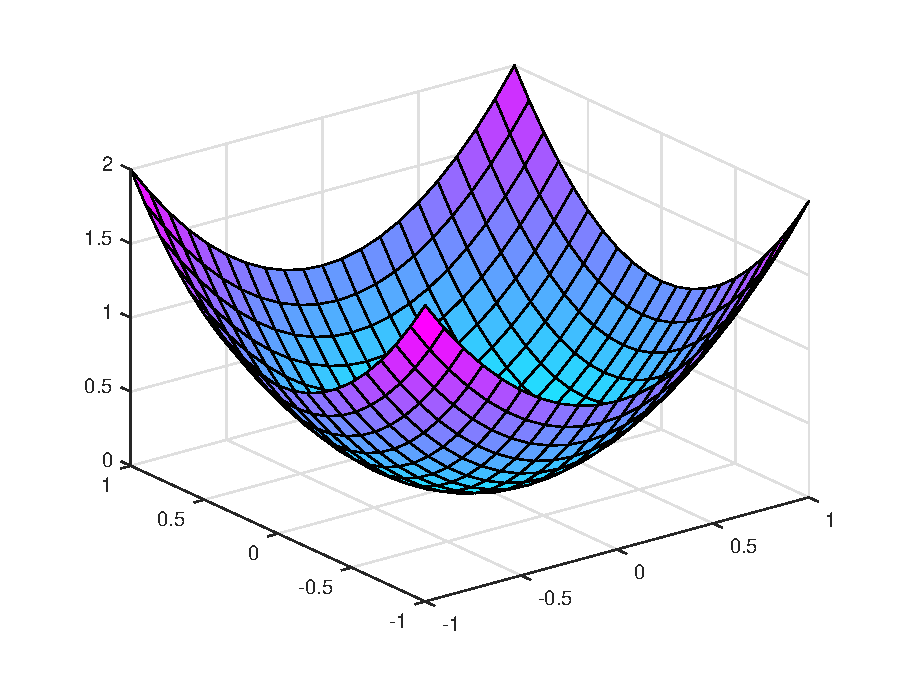
\includegraphics[width=.45\linewidth]{figs/g1}
	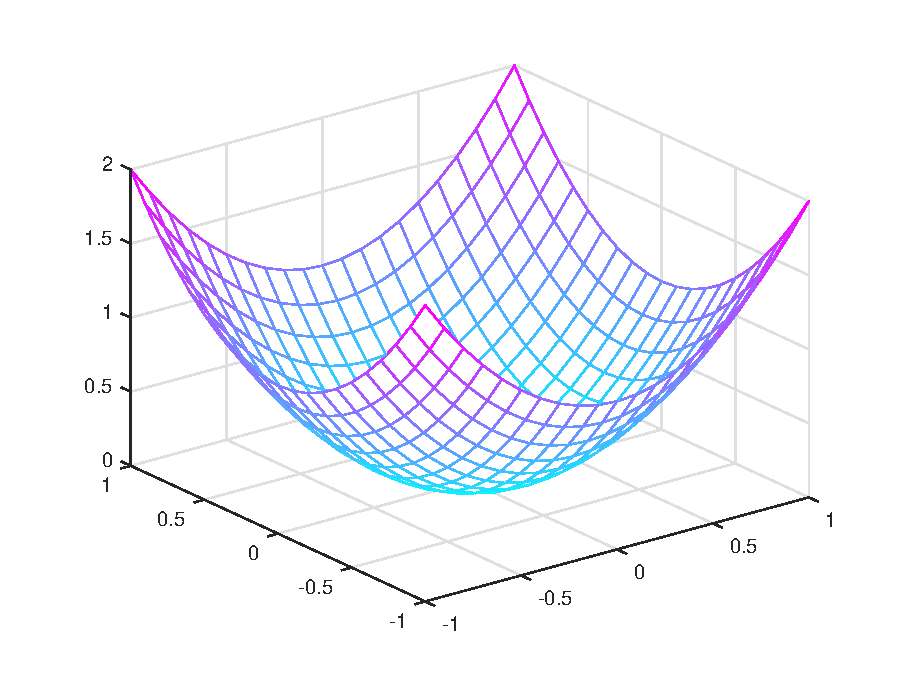
\includegraphics[width=.45\linewidth]{figs/g2}
	\caption{Exemplo de Figuras Vetorizadas}
\end{figure}

Há, quando for utilizar figuras em formato .eps, adicione no cabeçalho:
\begin{verbatim}
\usepackage[dvips]{graphicx}
\end{verbatim}

Obs: Neste template, este \textit{usepackage} já vem por padrão.

\subsection{Vantagem das Figuras vetorizadas}
Algumas das vantagens de figuras vetorizadas são:
\begin{itemize}
	\item Maior qualidade;
	\item Possibilidade de utilizar bastante \textit{zoom};
	\item Grande quantidade de detalhes.
\end{itemize}

\section{Aspas}

Você pode escrever texto em aspas simples desse modo:
\begin{verbatim}
  `texto entre aspas simples'
\end{verbatim}

Veja o resultado:
`texto entre aspas simples'\\

Já textos em aspas duplas podem ser feitas dessa forma
\begin{verbatim}
  ``texto entre aspas duplas''.
\end{verbatim}

Veja: ``texto entre aspas duplas''

\section{Cálculo Diferencial e Integral}

\subsection{Integrais}
Você pode fazer uma integral no \LaTeX dessa forma (em ambiente matemático, claro):
\begin{verbatim}
\int_{0}^{\infty} \frac{1}{x^2}.
\end{verbatim}

Veja o resultado:
\begin{equation}
\int_{0}^{\infty} \frac{1}{x^2}.
\end{equation}


\subsection{Limites}
Já para limites:
\begin{verbatim}
\lim_{x \to \infty}f(x)
\end{verbatim}

Veja o resultado:
\begin{equation}
\lim_{x \to \infty}f(x)
\end{equation}

\subsection{Exercício:}
Agora que fizemos juntos limites e derivadas, reproduza a seguinte definição:
$$
\int_{-\infty}^{+\infty}f(x)dx = \lim_{a \to -\infty}f(x) + \lim_{b \to +\infty}f(x).
$$

\section{Derivadas parciais}
$$
\frac{\partial z}{\partial t} = \frac{\partial z}{\partial x}\frac{\partial x}{\partial t} + \frac{\partial z}{\partial y}\frac{\partial y}{\partial t}
$$
Dica$^1$:
\begin{verbatim}
\frac{a}{b}
\end{verbatim}

Dica$^2$:
\begin{verbatim}
\partial
\end{verbatim}

\IEEEpeerreviewmaketitle


\bibliographystyle{plain} 
\bibliography{refs/library-references}


\end{document}
